\documentclass{beamer}
\usepackage[utf8]{inputenc}
\usepackage[T1]{fontenc}
\usepackage{eurosym}
\usepackage{rotating}
\usepackage{comment}
\usepackage{tikz}
\usepackage{pgf-umlcd}
\usetikzlibrary{arrows,automata,shapes}
\AtBeginSection[]
{
  \begin{frame}
  \frametitle{Wir sind hier:}
    \tableofcontents[currentsection]
  \end{frame}
}

\begin{document}

\title{Erkennen eines Graphen aus einer Punktwolke}
\date{}

\frame{\titlepage}

\section{Einleitung}
\frame{\frametitle{Das Problem}
\begin{description}
\item[Eingabe] ein metrischer Raum $(X, d)$, z.B.
  \begin{enumerate}
  \item GPS-Koordinaten eines Autos, das in einer Stadt herumfährt
  \item Koordinaten der schwarzen Pixel in einem Schwarz-Weiß-Bild
  \end{enumerate}
\item[Ausgabe] eine Approximation des metrischen Graphen, der dem metrischen Raum zugrunde liegt, z.B.
  \begin{enumerate}
  \item das Straßennetz der Stadt
  \item der Graph, der im Bild abgebildet wird\\ $\rightarrow$ Schrifterkennung
  \end{enumerate}
\end{description}
}

\frame{\frametitle{Wozu ist das nützlich?}

\begin{enumerate}
\item Struktur in gro{\ss}e Mengen geometrischer Daten bringen um deren Analyse zu ermöglichen/erleichtern \pause
\item Häufig enthalten die Daten rauschen und sind umfangreich $\rightarrow$ Ziel: Datenmenge kompakt in ihren wichtigsten Verzweigungen darstellen
\end{enumerate}
}

\frame{\frametitle{Beispiel (Erdbeben)}
\begin{figure}
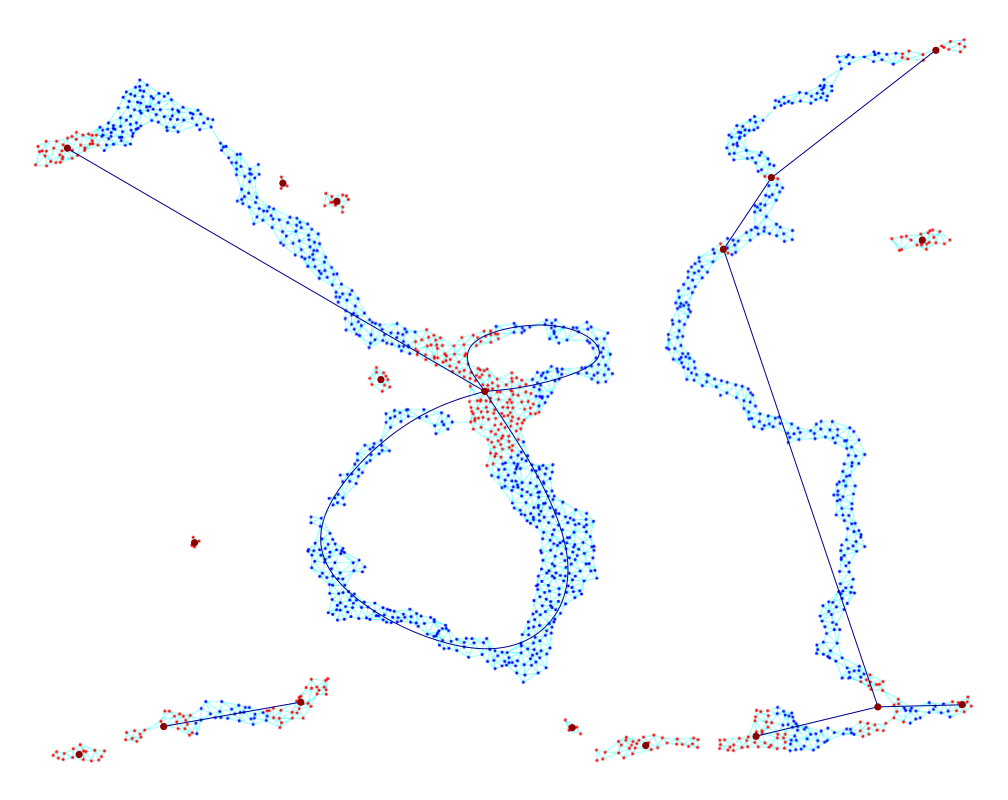
\includegraphics{images/faultlines.png}
\end{figure}
}

\frame{\frametitle{Beispiel (Straßennetz)}
\begin{figure}
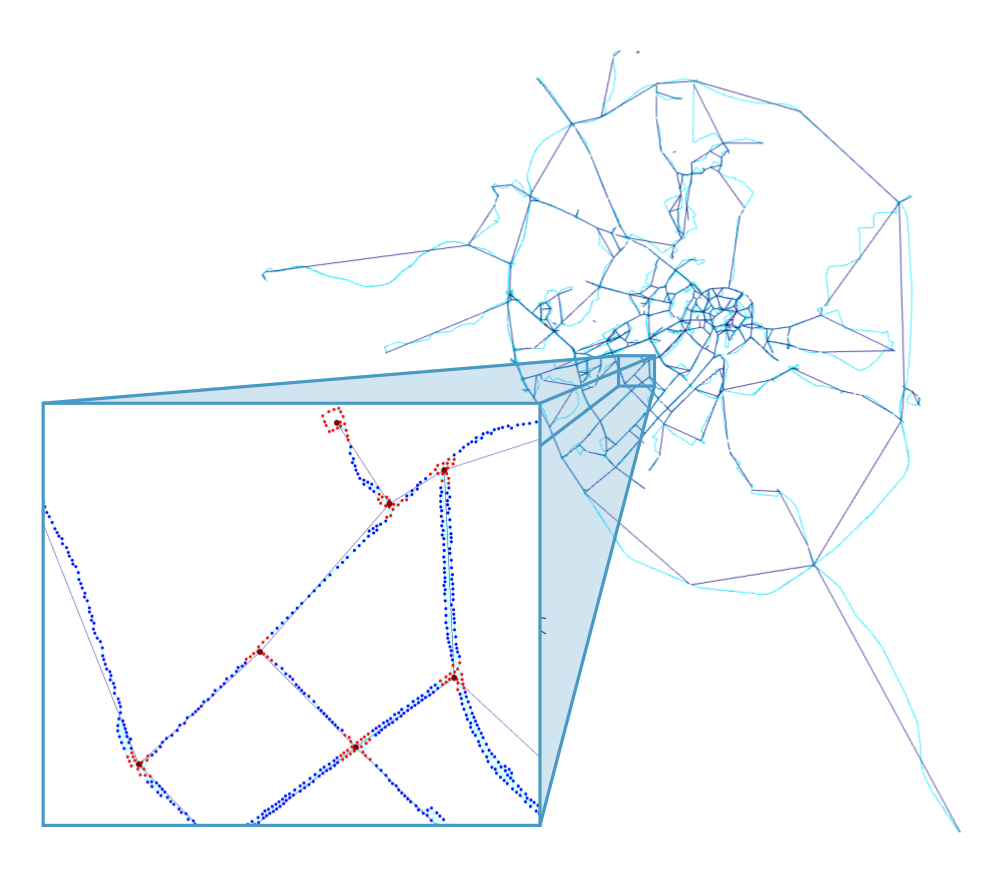
\includegraphics{images/roadnetwork.png}
\end{figure}
}

\section{Der Algorithmus}
\subsection{Der Algorithmus}
\frame{\frametitle{Drei wesentliche Schritte}
\begin{enumerate}
	\item[1] \textbf{Labeling}: Welche Punkte gehören zu Kanten, welche zu Knoten? $\rightarrow$ Punkte mit entsprechendem Label versehen\pause
	\item[2] \textbf{Rekonstruktion}: Anhand der Labels bestimmen, welche Punkte sich zu einem Knoten und welche sich zu einer Kante zusammentun $\rightarrow$ Rekonstruktion des der Punktmenge zugrundeliegenden Graphen\pause
	\item[3] \textbf{Metrik wiederherstellen}: Kanten mit Abständen versehen
\end{enumerate}
}

\frame{\frametitle{Zu Schritt 1: Labeling}
\begin{enumerate}
\item Betrachten einen kreisförmigen Ausschnitt um jeden Punkt und bestimmen Anzahl der Zusammenhangskomponenten darin
\begin{figure}
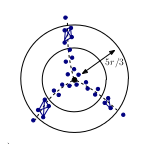
\includegraphics[height=2cm,width=2cm,keepaspectratio]{images/rips1.png}
\end{figure}
	\begin{itemize}
		\item Grad des Punkts = \# Zusammenhangskomponenten im kreisförmigen Ausschnitt
	\end{itemize}\pause
\item Grad == 2 $\rightarrow$ \textit{edge point} (wird später zu einer Kante gehören)\pause
\item Grad != 2 $\rightarrow$ \textit{preliminary branch point} (wird später zu einem Knoten gehören, aber noch umbenannt zu \textit{branch point})\pause
\item Alle weniger als $x$ von einem \textit{preliminary branch point} entfernten Punkte werden als \textit{branch points} eingeordnet (Knoten)
\end{enumerate}
}

\frame{\frametitle{Zu Schritt 2: Rekonstruktion des Graphen}
\begin{enumerate}
	\item Mithilfe der Labels bestimmen, welche Punkte sich zu einem Knoten und welche sich zu einer Kante zusammentun\pause
	\begin{itemize}
		\item Punkte sind jetzt nach dem Labeling in zwei Mengen aufgeteilt:
		\begin{itemize}
		\item \textit{edge points}
		\item \textit{branch points}
		\end{itemize}\pause
\item Um die Anzahl der späteren Kanten und Knoten zu bestimmen, wird Rips-Vietoris-Graph für beide Mengen erstellt\pause
	\begin{itemize}
		\item Im Rips-Vietoris-Graphen werden alle Punkte, die innerhalb eines gewissen Abstands zueinander liegen, zu einer Zusammenhangskomponente gefasst
    \end{itemize}\pause
\item Jede Zusammenhangskomponente entspricht einem Knoten, bzw. einer Kante\pause
\item Zwei Punkte werden durch eine Kante verbunden, wenn sie Punkte in ihrer Zusammenhangskomponente haben, die einen gewissen Abstand zu Punkten in der selben Zusammenhangskomponente einer Kante nicht überschreiten
	\end{itemize}
\end{enumerate}
}


\frame{\frametitle{Zu Schritt 3: Metrik wiederherstellen}
\begin{enumerate}
	\item Kanten mit Abständen versehen
	\begin{itemize}
		\item Jeder Kante wird als Länge der Durchmesser (längster kürzester Weg) ihrer Zusammenhangskomponente zugewiesen
	\end{itemize}
\end{enumerate}
}
\end{document}
